%  Pt1.tex
% !TeX spellcheck = en_GB
% !TeX root = ProjectRiskManagement.tex

\section{Approaches to Uncertainty and Underlying Complexity Management - 1200}

%Introduction to risk and opportunity, underlying complexity. 

%Challenge of traditional view of risk.
The phrasing ``uncertainty and underlying complexity management'' has been specifically selected as the title of this section to contrast with the risk management title of the the course as a whole.
Traditional views of risk management offer a very limited scope and an incomplete picture.
Often the focus is on event uncertainty reflecting the standard dictionary definition of risk: \textit{a hazard, chance of bad consequences, exposure to mischance} \citep{OED}.
This approach does not adequately address the whole of the uncertainty effecting the project, and in the worst case can lead to severe mismanagement and failed delivery of project objectives.
The Performance Uncertainty Management Process (PUMP) framework encourages departure from the project-centric approach advocated by best practice, to consider all corporate, operational and planning sources of uncertainty.
This expanded field of view allows the capture of ambiguity uncertainty, inherent variability, systematic uncertainty, as well as event uncertainty.
Using the PUMP framework shifts the focus of risk management to the achievement of opportunity efficiency and risk efficiency, through the vehicle of uncertainty management.

% execution and delivery strategy shaping phase of a project's life cycle
Procedures are a common way to ensure consistency and quality is maintained through a range of repeated applications.
While a good procedure is often designed to be simple, repeatable and transparent, this cannot be a uniform approach.
Some high complexity, high uncertainty projects require sophisticated, tailored procedures.
The PUMP framework supports this concept through the idea of PUMP packs, that is a set of PUMPs tailored to specific projects and project lifecycle stages.
Particularly, this paper focusses on PUMPs within the context of the E\&D strategy shaping stage.

%Project life cycle introduction.
A traditional four stage view of the asset/change lifecycle is a useful starting point to consider the scope of a project.
The four stages are conceptualize, planning, execution and delivery (E\&D) and Utilization.
As explained, effective uncertainty management requires a macro-view of the entire project to capture the whole of the uncertainty.
This leads to an elaboration of the lifecycle to incorporate 12 stages, each emphasizing a different management purpose and outcome.
Both views are shown in figure \ref{Figure:Project_Lifecycle}.

\begin{figure}[!h]
  \centering
    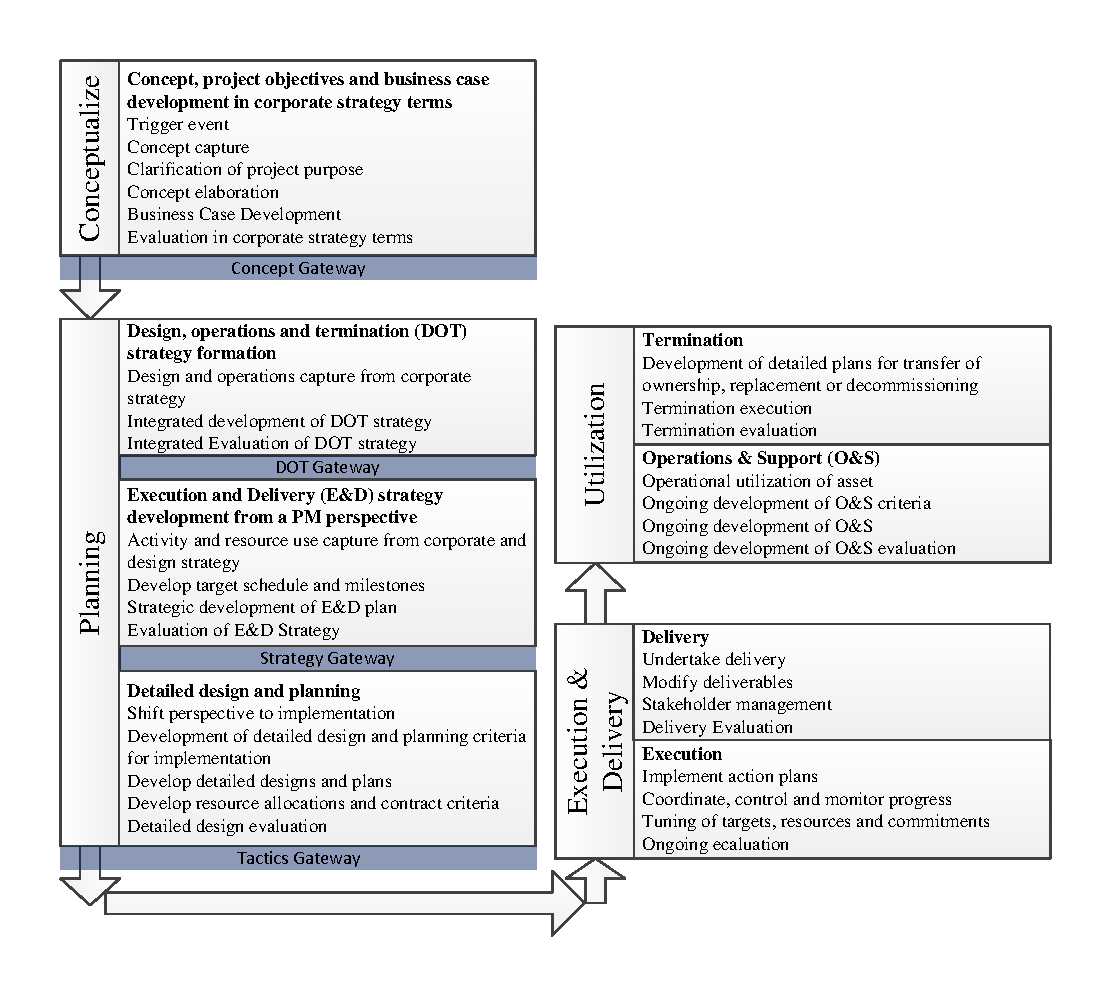
\includegraphics[width = \textwidth]{./Figures/ProjectLifecycleDetailedCurve.pdf} 
\caption{Twelve-stage asset/change lifecycle - adapted from \cite{chapman}}
\label{Figure:Project_Lifecycle}
\end{figure}

The planning stage of the traditional lifecycle is expanded to three shaping stages and three governance stages.
The design, operations and termination (DOT) stage aims to derive a strategy for DOT from the corporate strategy developed in the conceptualize stage.
A basic set of design criteria are built, and the objectives of the project are refined. 
Integrated evaluation is important to ensure non-viable projects are halted before large expenditure.
The execution and delivery (E\&D) strategy shaping stage takes a form more familiar in traditional project management.
The activity and resource requirements are derived from the corporate strategy and the DOT strategy.
This stage considers aspects of the project execution and asks how the asset/change will be delivered?
Schedule derivation takes place in the E\&D stage, including the reconciliation of corporate expectation and real-world plausibility.
Again, integrated evaluation is vital to ensuring only viable projects proceed to later more expensive stages of the lifecycle.
This paper is concerned with PUMPs particularly tailored to this cycle.



\subsection{The PUMP Process}
%Explain concisely in your own words what you believe are the key overall features of a PUMP approach to project risk management in the execution and delivery strategy shaping phase of a project’s lifecycle. Compare these features with the PMI PIMBOK approach or any other form of common practice you are familiar with if you find this helpful, but focus on the PUMP approach. Use examples to illustrate your discussion if you wish, but concentrate on concepts and principles. This will be a largely descriptive summary of your interpretation of the lectures and associated reading. It will demonstrate your grasp of the central core of the unit’s material as a whole, and should be approached with a view to demonstrating this understanding..

The generic PUMP process is a seven stage iterative cycle as shown in figure \ref{Figure:Project_Lifecycle}. 
An iterative approach allows the achievement of clarity efficiency.
The 80:20 rule empirically states that 20\% of the uncertainty causes 80\% of the risk. 
The first iteration of the PUMP is a high level sweep to identify the key areas of concern.
Subsequent iterations focus on these aspects until a sufficient level of clarity is achieved.

\begin{figure}[!h]
  \centering
\subfigure[Flowchart Visualisation]{
    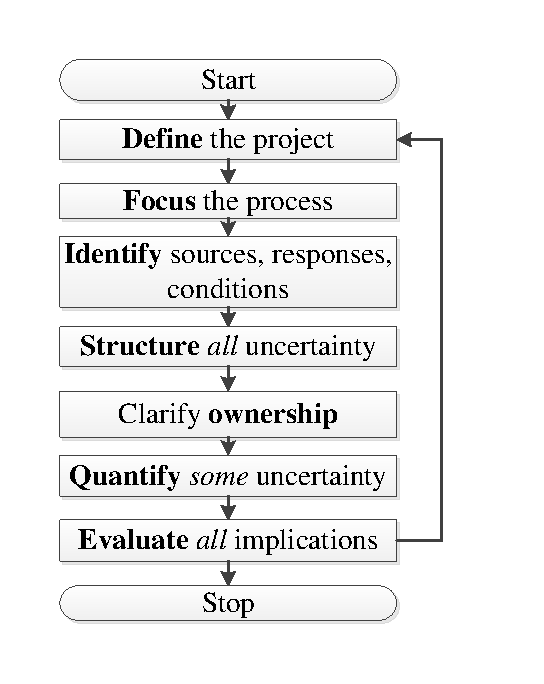
\includegraphics[height = 6cm]{./Figures/PUMPgeneric.pdf} 
	\label{Figure:GenericPUMP_Flow}
   } \quad
\subfigure[Gantt Chart Visualisation]{
    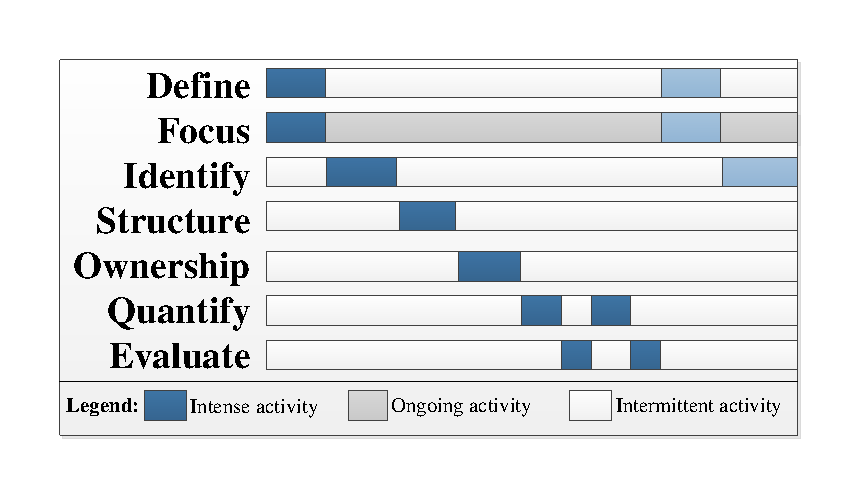
\includegraphics[height = 6cm]{./Figures/PUMPgenericGantt.pdf} 
	\label{Figure:GenericPUMP_Gantt}
   }
\caption{The generic PUMP process - adapted from \cite{chapman}}
\label{Figure:GenericPUMP_Both}
\end{figure}

The define phase \dots

The focus phase \dots

The identify phase \dots This phase is further elaborated in section \ref{}.

The structure phase \dots

The ownership phase \dots

The evaluate phase \dots This phase is further elaborated in section \ref{}.

\subsection{Contrast with Other Risk Management Processes}
Contrast with PUMP and PMI PMBOK and others.

\subsection{The Clarity Efficient Approach}
Summarise that PUMPS offer a higher level of clarity for the project as a whole rather than 


1200words.